\documentclass[oneside,11pt,parskip=half,ngerman]{scrreprt}
%\documentclass[a4paper,oneside,11pt,parskip=half,ngerman]{scrreprt}
\usepackage{typearea}

\usepackage[ngerman]{babel}
\usepackage[colorlinks=false, pdfborder={0 0 0}]{hyperref}
\usepackage{multirow}
\usepackage{booktabs}
\usepackage[utf8]{inputenc}
\usepackage[T1]{fontenc}
\usepackage{charter}
\usepackage[expert]{mathdesign}

\usepackage{listings}
\usepackage{xcolor}
\usepackage{color}
\usepackage{fancyhdr}
\usepackage{rotating}
\usepackage{titlesec}
\usepackage{mathptmx}
\usepackage{amssymb} % checkmark
% \usepackage{helvet}
\usepackage[scaled]{uarial}
\renewcommand*\familydefault{\sfdefault} %% Only if the base font of the document is to be sans serif
\usepackage[squaren]{SIunits}
\usepackage{graphicx}
\usepackage{url}
\usepackage{geometry}
\usepackage[absolute]{textpos}
\usepackage{makeidx}
\usepackage{colortbl}
\usepackage{pdflscape}
\usepackage{pdfpages}
\usepackage{tabularx}
\usepackage{lmodern}
\usepackage{longtable}
\usepackage{array}
\usepackage{float}
\usepackage{scrhack}
\usepackage{fancyhdr}
\usepackage{fancyvrb}

\usepackage[section]{placeins}

\usepackage{pdfpages}

\usepackage[firstpage]{draftwatermark}

%Typesetting
\usepackage[activate=true,final,tracking=true,kerning=true,spacing=true,factor=1100,stretch=10,shrink=10]{microtype}
\SetProtrusion{encoding={*},family={bch},series={*},size={6,7}}
              {1={ ,750},2={ ,500},3={ ,500},4={ ,500},5={ ,500},
               6={ ,500},7={ ,600},8={ ,500},9={ ,500},0={ ,500}}

% Bibliography
\usepackage[backend=bibtex]{biblatex}
\usepackage{csquotes}
\bibliography{./Citer}


%define page margin
\geometry{a4paper, top=30mm, left=30mm, right=30mm, bottom=30mm,headsep=10mm,footskip=10mm}

\usepackage{tocloft}
\setlength\cftbeforetoctitleskip{-2.5em}
\setlength\cftbeforeloftitleskip{-2.5em}
\setlength\cftbeforelottitleskip{-2.5em}




\usepackage{graphicx}
% We will generate all images so they have a width \maxwidth. This means
% that they will get their normal width if they fit onto the page, but
% are scaled down if they would overflow the margins.
\makeatletter
\def\maxwidth{\ifdim\Gin@nat@width>\linewidth\linewidth
\else\Gin@nat@width\fi}
\makeatother
\let\Oldincludegraphics\includegraphics
\renewcommand{\includegraphics}[1]{\Oldincludegraphics[width=\maxwidth,height=20em,keepaspectratio]{#1}}


% Chapter styling
\usepackage[grey]{quotchap}
\makeatletter 
\renewcommand*{\chapnumfont}{%
  \usefont{T1}{\@defaultcnfont}{b}{n}\fontsize{80}{100}\selectfont% Default: 100/130
  \color{chaptergrey}%
}
\makeatother

\begin{titlepage}
\title{\bigskip \bigskip }
\author{}

%\include{../content/Titelblatt.tex}
%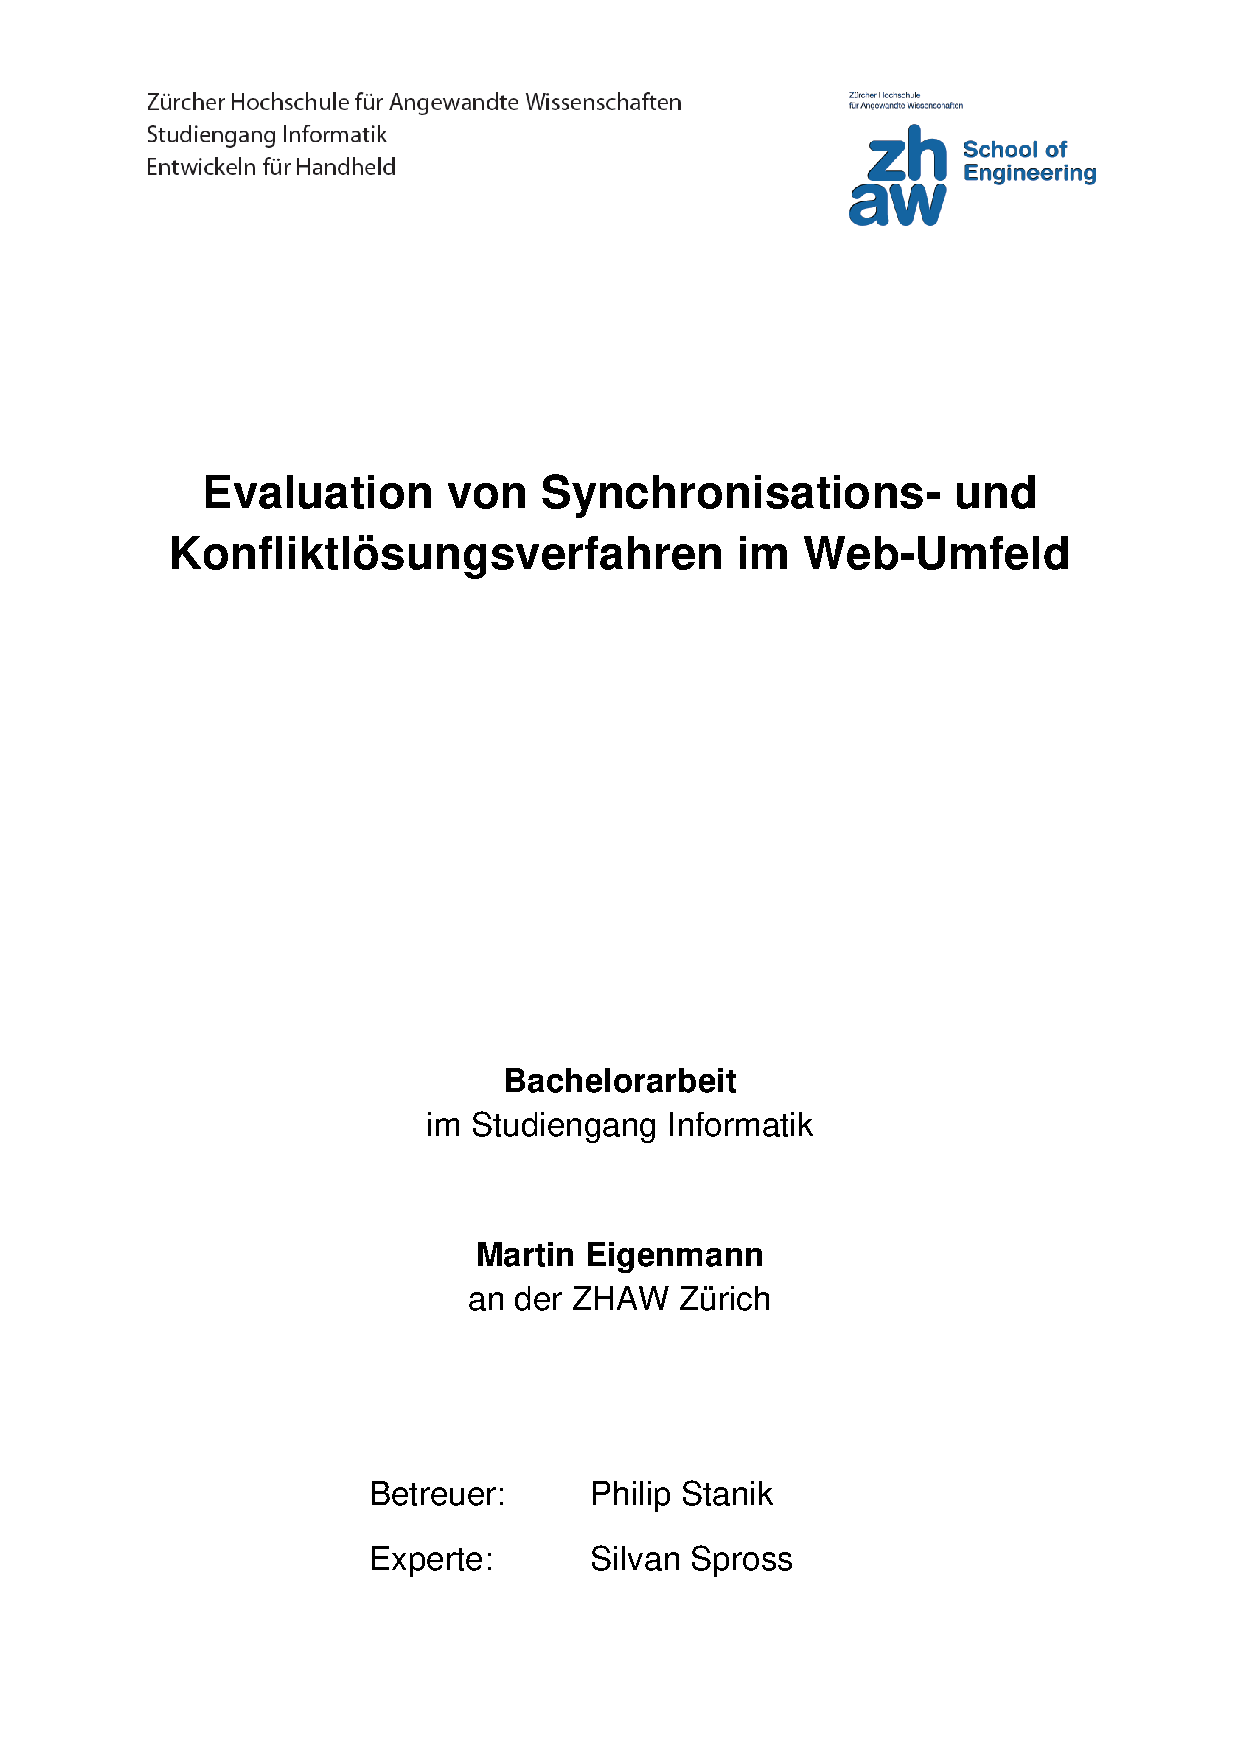
\includepdf[pages=1]{../content/Titelblatt}

\end{titlepage}

\begin{document}  
\maketitle

\chapter{Einleitung}\label{einleitung}

\section{Motivation und
Fragestellung}\label{motivation-und-fragestellung}

Der Zugriff auf Services und Medien mittels mobiler Geräte steigt
beständig an. So ist im Mai 2014, 60\% der Zeit, die online verbracht
wird, über Handy und Tablet zugegriffen worden - davon 51\% mittels
mobiler Applikationen. \autocite{comescore-mobiletrends}

\begin{figure}[htbp]
\centering
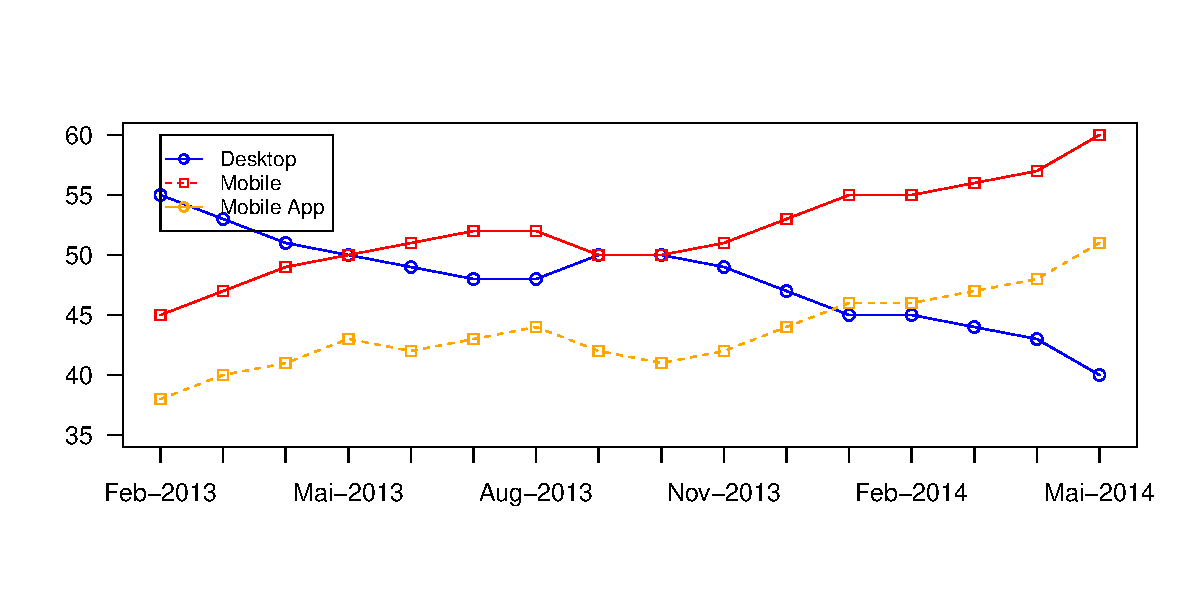
\includegraphics{img/Share-of-US-Digital-Media-Time-Spent-by-Platform.pdf}
\caption{Verteilung der online verbrachten Zeit nach Platform (Grafik
erstellt gemäss der Daten von \autocite{comescore-mobiletrends})}
\end{figure}

Angesichts der grossen Verbreitung und Nutzung von Services und Medien
im Internet, wird eine unterbruchsfreie Benutzbarkeit, auch ohne
Internetverbindung, immer selbstverständlicher und somit auch immer
wichtiger.

\begin{quote}
\enquote{It's clear that the mobile industry has finally given up on the
fantasy that an Internet connection is available to all users at all
times. Reality has set in. And in the past month, we've seen a new wave
of products and services that help us go offline and still function.}
\textcite{cw-mobiletrends}
\end{quote}

Es stellt sich nun die Frage, wie Informationen, über
Verbindungsunterbrüche hinweg, integer gehalten werden können. Und wie
Daten im mobilen Umfeld synchronisiert, aktualisiert und verwaltet
werden könne, so dass für den Endbenutzer schlussendlich kein
Unterschied zwischen Online- und Offline-Betrieb mehr wahrnehmbar ist.

\section{Aufgabenstellung}\label{aufgabenstellung}

Die von der Leitung des Studiengangs Informatik freigegebene
Aufgabenstellung ist im Appendix unter
\enquote{\hyperref[appendixux5faufgabenstellung]{Aufgabenstellung}}
aufgeführt.

\section{Abgrenzung der Arbeit}\label{abgrenzung-der-arbeit}

\section{Begründung}\label{begruxfcndung}

\section{Geschichtliche Einordnung in das
Thema}\label{geschichtliche-einordnung-in-das-thema}

\chapter{Dokumentationsstruktur und Beitrag zum
Forschungsgebiet}\label{dokumentationsstruktur-und-beitrag-zum-forschungsgebiet}

\emph{Teil i - Einleitung und Abgrenzung}

\emph{Teil ii - Technische Grundlagen und Architekturen}

\emph{Teil iii - Konzept und Implementierung}

\emph{Teil iv - Abschluss und Ausblick}

\chapter{Recherche}\label{recherche}

Dieses Kapitel erklärt die wichtigsten Grundbegriffe und wiedergibt die
während der Recherche gesammelten Informationen.

\section{Fachbegriffe}\label{fachbegriffe}

Eine Aufführung und Erlährung der Fachbegriffe befindet sinch im
Appendix unter \enquote{{[}Glossar{]}}

\section{Erläuterung der
Grundlagen}\label{erluxe4uterung-der-grundlagen}

\subsection{Datenbanken}\label{datenbanken}

Eine Datenbank \footnote{In der Literatur oft auch als
  \textbf{D}aten\textbf{B}ank\textbf{S}ystemen (DBS) oder
  Informationssystem bezeichnet. \autocite[ pp.~3-4]{rupDatenbanken}}
ist ein System zur Verwaltung und Speicherung von strukturierten Daten.
Erst durch den Kontext des Datenbankschemas wird aus den Daten
Informationen, die zur weiteren Verarbeitung genutzt werden können. Ein
Datenbanksystem umfasst die beiden Komponenten Datenbankmanagementsystem
(DBMS) sowie die zu veraltenden Daten selbst.\\Ein DBMS muss die vier
Aufgaben \footnote{Bekannt als ACID-Prinzip \autocite[
  pp.105]{rupDatenbanken} umfasst es \textbf{A}tomicity,
  \textbf{C}onsistency, \textbf{I}solation und \textbf{D}urability.}
erfüllen.

\begin{itemize}
\itemsep1pt\parskip0pt\parsep0pt
\item
  Atomarität
\item
  Konsistenzerhaltung
\item
  Isolation
\item
  Dauerhaftigkeit
\end{itemize}

Neben den vielen neu auf den Markt erschienen Technologien wie Document
Store oder Key-Value Store ist das Relationale Datenbankmodell immer
noch am verbreitetsten. \autocite{dbenginesranking}.

\subsection{Monolithische Systeme}\label{monolithische-systeme}

Als Monolithisch wird ein logisches System bezeichnet, wenn es in sich
geschlossen, ohne Abhängigkeiten zu anderen Systemen operiert. Alle zur
Erfüllung der Aufgaben benötigten Ressourcen sind im System selbst
enthalten. Es müssen also keine Ressourcen anderer Systeme alloziert
werden und somit ist auch keine Kommunikation oder Vernetzung
notwendig.\\Das System selbst muss jedoch nicht notwendigerweise aus nur
einem Rechenknoten bestehen, sondern darf auch als Cluster implementiert
sein.

\subsection{Verteilte Systeme}\label{verteilte-systeme}

Man kann zwischen physisch und logisch verteilten Systemen
unterscheiden. Weiter kann das System auf verschiedenen
Abstraktionsstufen betrachtet werden. So sind je nach Betrachtungsvektor
unterschiedliche Aspekte relevant und interessant.
\autocite{ethdistribsystems}

\subsubsection{physisch verteilte
Systeme}\label{physisch-verteilte-systeme}

Rechnernetze und Cluster-Systeme werden typischerweise als physisch
verteiltes System betrachtet. Die Kommunikation zwischen den einzelnen
Rechenknoten erfolgt Nachrichten orientiert und ist somit asynchron
ausgelegt. Jeder Rechenknoten verfügt über exklusive Speicherressourcen
und einen eigenen Zeitgeber.\\Durch die Implementation eines Systems
über mehrere unabhängige physische Rechenknoten kann eine erhöhte
Ausfallsicherheit und/oder ein Performance-Gewinn erreicht werden.

\subsubsection{logisch verteilte
Systeme}\label{logisch-verteilte-systeme}

Falls innerhalb eines Rechenknoten echte Nebenläufigkeit\footnote{Von
  echter Nebenläufigkeit wird gesprochen, wenn verschiedene Prozesse zur
  selben Zeit ausgeführt werden. (Multiprozessor)} oder
Modularität\footnote{Modularität beschreibt die Unabhängigkeit und
  Austauschbarkeit einzelner (Software-) Komponenten. (Auch Lose
  Kopplung gennant)} erreicht wird, kann von einem logisch verteilten
System gesprochen werden. Einzelne Rechenschritte und Aufgaben werden
unabhängig voneinander auf der selben Hardware ausgeführt. Dies
ermöglicht den flexiblen Austauschen\footnote{Austauschbarkeit einzelner
  Programmteile wird durch die Einhaltung der Grundsätze von modularer
  Programmierung erreicht.} einzelner Aufgaben.

\subsection{Verteilte Algorithmen}\label{verteilte-algorithmen}

Verteilte Algorithmen sind Prozesse welche miteinander über Nachrichten
(synchron oder asynchron) kommunizieren und so idealerweise ohne
Zentrale Kontrolle eine Kooperation erreichen.
\autocite{ethdistribalgo}\\Performance-Gewinn, bessere Skalierbarkeit
und eine breitere Abdeckung der unterstützen von verschiedenen
Hardware-Architekturen kann durch den Einsatz von verteilten Algorithmen
erreicht werden.

\subsection{Verteilte Datenbanken}\label{verteilte-datenbanken}

{[}Präsenzbibliothek ZHAW{]}

\subsection{Replikation}\label{replikation}

Replikation vervielfacht ein sich möglicherweise mutierendes Objekt
(Datei, Dateisystem, Datenbank usw.), um hohe Verfügbarkeit, hohe
Performance, hohe Integrität oder eine beliebige Kombination davon zu
erreichen. \autocite[ p.~19]{SWB-327013990}

\hyperdef{}{synchrone-replikation}{\subsubsection{Synchrone
Replikation}\label{synchrone-replikation}}

Eine synchrone Replikation stellt sicher, dass zu jeder Zeit der gesamte
Objektbestand auf allen Replikationsteilnehmern identisch ist.

Wird ein Objekt eines Replikationsteilnehmer mutiert, wird zum
erfolgreichen Abschluss dieser Transaktion, von allen anderen
Replikationsteilnehmern verlangt, dass sie diese Operation ebenfalls
erfolgreich abschliessen.\\Üblicherweise wird dies über ein
Primary-Backup Verfahren realisiert. Andere Verfahren wie der
2-Phase-Commit und 3-Phase-Commit ermöglichen darüber hinaus auch das
editieren von Objekten auf allen Replikationsteilnehmern. \autocite[
p.~23ff, 134ff]{SWB-327013990}

\subsubsection{Asynchrone Replikation}\label{asynchrone-replikation}

Eine asynchrone Replikation, stellt periodisch sicher, dass der gesamte
Objektbestand auf allen Replikationsteilnehmern identisch ist.
Mutationen können nur auf dem Master-Knoten durchgeführt werden. Einer
oder mehrere Backup-Knoten übernehmen dann periodisch die
Mutationen.\\Entgegen der \hyperref[synchrone-replikation]{synchronen
Replikation} müssen nicht alle Replikationsteilnehmer zu jedem Zeitpunkt
verfügbar sein\footnote{So kann der Backup-Knoten nur Nachts über
  verfügbar sein, damit die dazwischen liegende Verbindung Tags über
  nicht belastet wird.}.

\subsubsection{Merge Replikation}\label{merge-replikation}

Die merge Replikation erlaubt das mutieren des Objekts auf allen
Replikationsteilnehmern.\\Mutationen an einem einzelnen
Replikationsteilnehmer werden allen übrigen Replikationsteilnehmern
mitgeteilt. Da ein Objekt zwischenzeitlich\footnote{Zwischen der lokalen
  Mutation und der Publikation dieser an die übrigen
  Replikationsteilnehmer, liegt eine beliebige Latenz.} auch auf anderen
Teilnehmern mutiert worden sein kann, müssen während des
Synchronisationsvorgang\footnote{Da die Replikation nicht
  notwendigerweise nur unidirektional, sondern im Falle von einem
  Multi-Master Setup auch bidirektional durchgeführt werden kann, wird
  hier von einer Synchronisation gesprochen.} eventuell auftretenden
Konflikte aufgelöst werden.

\subsection{Block-Chain}\label{block-chain}

Die Block-Chain ist eine verteilte Datenbank die ohne Zentrale Kontrolle
auskommt. Jede Transaktion wird kryptographisch gesichert, der Kette von
Transaktionen hinzugefügt. So ist das entfernen oder ändern
vorhergehender Einträge nicht mehr möglich\footnote{Das ändern
  vorhergehender Einträge benötigt mehr Rechenzeit, als alle anderen
  Teilnehmer ab diesem Zeitpunkt zusammen aufgewendet haben.}. Jeder
Teilnehmer darf also alle Einträge lesen und neue Einträge hinzufügen.
Da Einträge nur hinzugefügt werden und nie ein Eintrag geändert wird,
kann eine Block-Chain immer ohne Synchronisationskonflikte repliziert
werden. Konflikte können nur in den darüberlegenden logischen
Schichten\footnote{So prüft die Bitcoin-Implementation ob eine
  Transaktion (Überweisung eines Betrags) bereits schon einmal
  ausgeführt wurde, und verweigert gegebenenfalls eine erneute
  Ausführung.} auftreten. \autocite{block-chain}

\chapter{Analyse}\label{analyse}

\section{Datenanalyse}\label{datenanalyse}

\section{Diskussion bekannter
Verfahren}\label{diskussion-bekannter-verfahren}

\section{Anforderungsanalyse}\label{anforderungsanalyse}

\section{Vorgehensweise}\label{vorgehensweise}

\subsection{Use-Cases}\label{use-cases}

\subsection{Anforderungen}\label{anforderungen}

\subsection{Akzeptanzkriterien}\label{akzeptanzkriterien}

\subsection{Bewertung der
Anforderungen}\label{bewertung-der-anforderungen}

\section{Risiken}\label{risiken}

\chapter{Konzept}\label{konzept}

\section{Konfliktverhinderung}\label{konfliktverhinderung}

\subsection{2PC/3PC}\label{pc3pc}

\subsection{Block-Chain}\label{block-chain-1}

\subsection{Update Transformation}\label{update-transformation}

\section{Konfliktauflösung}\label{konfliktaufluxf6sung}

\subsection{Merge}\label{merge}

\subsection{Normalized Merge}\label{normalized-merge}

\subsection{Wiederholbare Transaktion}\label{wiederholbare-transaktion}

\subsection{Kausalitäts Merge}\label{kausalituxe4ts-merge}


\end{document}